\documentclass{article}

\usepackage{standalone}
\usepackage{basicreq}
\usepackage{./teaching_doc_macros}
\usepackage{amsmath}
\usepackage{tikz}
\usetikzlibrary{positioning}
\title{Lecture 1: Introduction}
\author{Shashank Vatedka}


\begin{document}

%FILL IN THE RIGHT INFO.
%\lecture{**LECTURE-NUMBER**}{**UNIT**}{**LECTURER**}{**SCRIBE**}
\lecture{6}{Review of information theoretic quantities}{Shashank Vatedka}{Kuntal Kokate}

\section{Data processing inequality}

\textbf{If $X-Y-Z$ forms a Markov chain,}
\begin{itemize}
    \item $I(X;Y) \geq I(X;Z)$
    \item $I(Y;Z) \geq I(X;Z)$
    \item $Pr_{Z|X,Y}(z|x,y) = Pr_{Z|Y}(z,y)$
    \item $Pr_{X|Y,Z}(x|y,z) = Pr_{X|Y}(x|y)$
\end{itemize} 

\section{Chain rule of entropy}
\begin{itemize}
    \item \begin{align}
        H(X;Y) & = H(X) + H(Y|X) \\
            & = H(Y) + H(X|Y)
    \end{align}
    \item \begin{align}H(X_1, X_2, ... ,X_n) = \sum_{i=1}^{\infty} H(X_i|X_1, X_2 ... , X_{i-1})\end{align}
\end{itemize}

\section{Chain rule of mutual information}
\begin{itemize}
    \item $I(X_1, X_2; Y) = I(X_1; Y) + I(X_2; Y| X_1)$
\end{itemize}


\section{Degraded Channels}

$\bfq_{Y|X}$ is stochastically degraded w.r.t. $\bfp_{Z|X}$ if we can find $\bfr_{Y|Z}$ such that,
    $$\bfq_{Y|X}(y|x) = \sum_{z \epsilon \bZ} \bfr_{Y|Z}(y|z)\bfp_{Z|X}(z|x)$$

If $C_{DMC1} \geq C_{DMC2} \implies$ channel 2 is degraded wrt channel 1.

\textbf{HW} If $I(X;Z) \geq I(X;Y)$, show that $C_{DMC1} \geq C_{DMC2}$ \newline
\textbf{Solution:}
\begin{align}
    & C = max_{\bfp_x} I(X;Y)  \\
    \implies & max_{\bfp_x}I(X;Z) \geq max_{\bfp_x}I(X;Y) \\
     \implies & C_{DMC1} \geq C_{DMC2}
\end{align}

\subsection{Capacity of channels}

\begin{itemize}
    \item $C_{BSC}(p) = 1 - H_2(p)$
    \item $C_{BEC}(p) = 1 - p$
    \item $C_{AWGN}(p, \sigma^2) =  \frac{1}{2}log(1 + \frac{p}{\sigma^2})$
\end{itemize}

\subsection{Examples}
\textbf{Problem 1.} Can BSC(0.1) be degraded wrt BSC(0.2) \\
\textbf{Solution} $$C_{BSC(0.1)} \ge C_{BSC(0.2)}$$
Therefore, BSC(0.2) is degraded wrt BSC(0.1)

\begin{figure}[!ht]
    \centering
    \documentclass{standalone}
\usepackage{tikz}
\usepackage{basicreq}

\usetikzlibrary{positioning}
\begin{document}

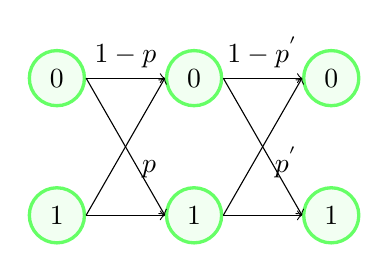
\begin{tikzpicture}[
roundnode/.style={circle, draw=green!60, fill=green!5, very thick, minimum size=7mm},
squarednode/.style={rectangle, draw=red!60, fill=red!5, very thick, minimum size=5mm},
]
%Nodes
\node[roundnode, label=above:{$\bfX$}]     (zero_1)                          {0};
\node[roundnode]       (one_1)       [below=of zero_1] {1};
\node[roundnode, label=above:{$\bfY$}]      (zero_2)       [right=of zero_1] {0};
\node[roundnode]       (one_2)       [below=of zero_2] {1};
\node[roundnode, label=above:{$\bfZ$}]      (zero_3)       [right=of zero_2] {0};
\node[roundnode]       (one_3)       [below=of zero_3] {1};

\draw[->] (zero_1.east) -- (zero_2.west) node[pos=0.5, sloped, above] {$1-p$};
\draw[->] (zero_2.east) -- (zero_3.west) node[pos=0.5, sloped, above] {$1-p^{'}$};
\draw[->] (one_1.east) -- (one_2.west);
\draw[->] (one_2.east) -- (one_3.west);
\draw[->] (zero_1.east) -- (one_2.west) node[pos=0.8, above] {$p$};
\draw[->] (zero_2.east) -- (one_3.west) node[pos=0.8, above] {$p^{'}$};
\draw[->] (one_1.east) -- (zero_2.west);
\draw[->] (one_2.east) -- (zero_3.west);

\end{tikzpicture}
\end{document}
    \caption{Combination of two BSC's}
    \label{fig:bsc}
\end{figure}

We can write the combination of two BSCs as one BSC($p \ast p^{'}$).
\begin{align}
    & p \ast p^{'} = p(1-p^{'}) + p^{'}(1-p) \\
    \implies & 0.1 = p^{'}(1-0.2) + (1-p^{'})0.2  \\
    \implies & p^{'} = 0.125
\end{align}

Therefore we can say that, BSC(0.2) is concantenation of BSC(0.1) and BSC(0.125).

\textbf{Problem 2.} BEC(0.1) vs BEC(0.2)\\
\textbf{Solution} $$C_{BEC(0.1)} \ge C_{BEC(0.2)}$$
Therefore, BEC(0.2) is degraded wrt BEC(0.1)
\begin{figure}[!ht]
    \centering
    \documentclass{standalone}
\usepackage{tikz}
\usepackage{basicreq}

\usetikzlibrary{positioning}
\begin{document}

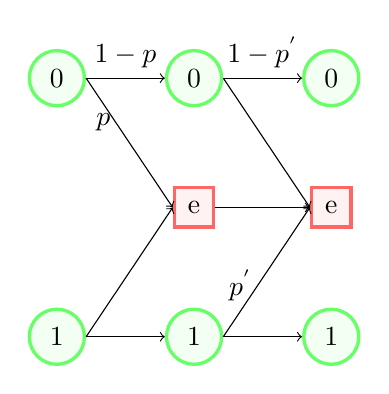
\begin{tikzpicture}[
roundnode/.style={circle, draw=green!60, fill=green!5, very thick, minimum size=7mm},
squarednode/.style={rectangle, draw=red!60, fill=red!5, very thick, minimum size=5mm},
]
%Nodes
\node[roundnode, label=above:{$\bfX$}]     (zero_1)                          {0};
\node[roundnode, label=above:{$\bfY$}]      (zero_2)       [right=of zero_1] {0};
\node[squarednode]       (e_2)       [below=of zero_2] {e};
\node[roundnode]       (one_2)       [below=of e_2] {1};
\node[roundnode]       (one_1)       [left=of one_2] {1};
\node[roundnode, label=above:{$\bfZ$}]      (zero_3)       [right=of zero_2] {0};
\node[squarednode]       (e_3)       [below=of zero_3] {e};
\node[roundnode]       (one_3)       [below=of e_3] {1};

\draw[->] (zero_1.east) -- (zero_2.west) node[pos=0.5, sloped, above] {$1-p$};
\draw[->] (zero_2.east) -- (zero_3.west) node[pos=0.5, sloped, above] {$1-p^{'}$};
\draw[->] (zero_1.east) -- (e_2.west)node[pos=0.2, below] {$p$};
\draw[->] (one_1.east) -- (e_2.west);
\draw[->] (one_1.east) -- (one_2.west);
\draw[->] (one_2.east) -- (one_3.west);
\draw[->] (e_2.east) -- (e_3.west);
\draw[->] (zero_2.east) -- (e_3.west);
\draw[->] (one_2.east) -- (e_3.west)node[pos=0.2, above] {$p^{'}$};

\end{tikzpicture}
\end{document}
    \caption{Combination of two BEC's}
    \label{fig:bec}
\end{figure}

\begin{align}
    & p^{''} = (1-p)p^{'} + p \\
    & 0.2 = (1-0.1)p^{'} + 0.1\\
    \implies & p^{'} = \frac{1}{9}
\end{align}

\textbf{Problem 3.} BSC(0.1) vs BEC(0.1)\\
\textbf{Solution} \begin{align}
    &C_{BEC(0.1)} = 0.9 \\
    &C_{BSC(0.1)} = 0.53
\end{align}
Therefore, BSC(0.1) is degraded wrt BEC(0.1).


\textbf{Problem 4.} BSC(0.01) vs BEC(0.5)\\
\textbf{Solution} \begin{align}
    &C_{BEC(0.5)} = 0.5 \\
    &C_{BSC(0.01)} \approx 1
\end{align}
    Therefore, BEC(0.5) is degraded wrt BSC(0.01).

\subsection{AWGN channels}
\textbf{Let $\sigma_{1}^2 \geq \sigma_{2}^2$, then $C_{1} \geq C_{2}$.
Therefore channel 2 is degraded wrt channel 1.} \\
There exist some $\sigma_{3}^2$ such that,
\begin{align}
    \sigma_{1}^2 = \sigma_{2}^2 + \sigma_{3}^2
\end{align}

\subsection{Uniform channels}
\textbf{Let $\alpha_{1} \geq \alpha_{2}$, then $C_{2} \geq C_{1}$.
Therefore channel 1 is degraded wrt channel 2.} \\
There exist some $\alpha_{3}$ such that,
\begin{align}
    \alpha_{1} = \alpha_{2} + \alpha_{3}
\end{align}
\end{document}


